% Template for PLoS
% Version 3.5 March 2018
%
% % % % % % % % % % % % % % % % % % % % % %
%
% -- IMPORTANT NOTE
%
% This template contains comments intended
% to minimize problems and delays during our production
% process. Please follow the template instructions
% whenever possible.
%
% % % % % % % % % % % % % % % % % % % % % % %
%
% Once your paper is accepted for publication,
% PLEASE REMOVE ALL TRACKED CHANGES in this file
% and leave only the final text of your manuscript.
% PLOS recommends the use of latexdiff to track changes during review, as this will help to maintain a clean tex file.
% Visit https://www.ctan.org/pkg/latexdiff?lang=en for info or contact us at latex@plos.org.
%
%
% There are no restrictions on package use within the LaTeX files except that
% no packages listed in the template may be deleted.
%
% Please do not include colors or graphics in the text.
%
% The manuscript LaTeX source should be contained within a single file (do not use \input, \externaldocument, or similar commands).
%
% % % % % % % % % % % % % % % % % % % % % % %
%
% -- FIGURES AND TABLES
%
% Please include tables/figure captions directly after the paragraph where they are first cited in the text.
%
% DO NOT INCLUDE GRAPHICS IN YOUR MANUSCRIPT
% - Figures should be uploaded separately from your manuscript file.
% - Figures generated using LaTeX should be extracted and removed from the PDF before submission.
% - Figures containing multiple panels/subfigures must be combined into one image file before submission.
% For figure citations, please use "Fig" instead of "Figure".
% See http://journals.plos.org/plosone/s/figures for PLOS figure guidelines.
%
% Tables should be cell-based and may not contain:
% - spacing/line breaks within cells to alter layout or alignment
% - do not nest tabular environments (no tabular environments within tabular environments)
% - no graphics or colored text (cell background color/shading OK)
% See http://journals.plos.org/plosone/s/tables for table guidelines.
%
% For tables that exceed the width of the text column, use the adjustwidth environment as illustrated in the example table in text below.
%
% % % % % % % % % % % % % % % % % % % % % % % %
%
% -- EQUATIONS, MATH SYMBOLS, SUBSCRIPTS, AND SUPERSCRIPTS
%
% IMPORTANT
% Below are a few tips to help format your equations and other special characters according to our specifications. For more tips to help reduce the possibility of formatting errors during conversion, please see our LaTeX guidelines at http://journals.plos.org/plosone/s/latex
%
% For inline equations, please be sure to include all portions of an equation in the math environment.  For example, x$^2$ is incorrect; this should be formatted as $x^2$ (or $\mathrm{x}^2$ if the romanized font is desired).
%
% Do not include text that is not math in the math environment. For example, CO2 should be written as CO\textsubscript{2} instead of CO$_2$.
%
% Please add line breaks to long display equations when possible in order to fit size of the column.
%
% For inline equations, please do not include punctuation (commas, etc) within the math environment unless this is part of the equation.
%
% When adding superscript or subscripts outside of brackets/braces, please group using {}.  For example, change "[U(D,E,\gamma)]^2" to "{[U(D,E,\gamma)]}^2".
%
% Do not use \cal for caligraphic font.  Instead, use \mathcal{}
%
% % % % % % % % % % % % % % % % % % % % % % % %
%
% Please contact latex@plos.org with any questions.
%
% % % % % % % % % % % % % % % % % % % % % % % %

\documentclass[10pt,letterpaper]{article}
\usepackage[top=0.85in,left=2.75in,footskip=0.75in]{geometry}

% amsmath and amssymb packages, useful for mathematical formulas and symbols
\usepackage{amsmath,amssymb}

% Use adjustwidth environment to exceed column width (see example table in text)
\usepackage{changepage}

% Use Unicode characters when possible
\usepackage[utf8x]{inputenc}

% textcomp package and marvosym package for additional characters
\usepackage{textcomp,marvosym}

% cite package, to clean up citations in the main text. Do not remove.
\usepackage{cite}

% Use nameref to cite supporting information files (see Supporting Information section for more info)
\usepackage{nameref,hyperref}

% line numbers
\usepackage[right]{lineno}

% ligatures disabled
\usepackage{microtype}
\DisableLigatures[f]{encoding = *, family = * }

% color can be used to apply background shading to table cells only
\usepackage[table]{xcolor}

% array package and thick rules for tables
\usepackage{array}

% create "+" rule type for thick vertical lines
\newcolumntype{+}{!{\vrule width 2pt}}

% create \thickcline for thick horizontal lines of variable length
\newlength\savedwidth
\newcommand\thickcline[1]{%
  \noalign{\global\savedwidth\arrayrulewidth\global\arrayrulewidth 2pt}%
  \cline{#1}%
  \noalign{\vskip\arrayrulewidth}%
  \noalign{\global\arrayrulewidth\savedwidth}%
}

% \thickhline command for thick horizontal lines that span the table
\newcommand\thickhline{\noalign{\global\savedwidth\arrayrulewidth\global\arrayrulewidth 2pt}%
\hline
\noalign{\global\arrayrulewidth\savedwidth}}


% Remove comment for double spacing
\usepackage{setspace}
\doublespacing

% Text layout
\raggedright
\setlength{\parindent}{0.5cm}
\textwidth 5.25in
\textheight 8.75in

% Bold the 'Figure #' in the caption and separate it from the title/caption with a period
% Captions will be left justified
\usepackage[aboveskip=1pt,labelfont=bf,labelsep=period,justification=raggedright,singlelinecheck=off]{caption}
\renewcommand{\figurename}{Fig}

% Use the PLoS provided BiBTeX style
\bibliographystyle{plos2015}

% Remove brackets from numbering in List of References
\makeatletter
\renewcommand{\@biblabel}[1]{\quad#1.}
\makeatother



% Header and Footer with logo
\usepackage{lastpage,fancyhdr,graphicx}
\usepackage{epstopdf}
%\pagestyle{myheadings}
\pagestyle{fancy}
\fancyhf{}
%\setlength{\headheight}{27.023pt}
%\lhead{\includegraphics[width=2.0in]{PLOS-submission.eps}}
\rfoot{\thepage/\pageref{LastPage}}
\renewcommand{\headrulewidth}{0pt}
\renewcommand{\footrule}{\hrule height 2pt \vspace{2mm}}
\fancyheadoffset[L]{2.25in}
\fancyfootoffset[L]{2.25in}
\lfoot{\today}

%% Include all macros below

\newcommand{\lorem}{{\bf LOREM}}
\newcommand{\ipsum}{{\bf IPSUM}}

%% END MACROS SECTION


%%%%%%%%%%%%%%%%%%%%% For Devan
% Reference
% 	See https://journals.plos.org/plosone/s/latex#loc-references
% 	On copy/paste, replace cite and cite with cite, remove square brackets


\begin{document}
\vspace*{0.2in}

% Title must be 250 characters or less.
\begin{flushleft}
{\Large
\textbf\newline{Assessing dependence between frequency and severity through shared
random effects} % Please use "sentence case" for title and headings (capitalize only the first word in a title (or heading), the first word in a subtitle (or subheading), and any proper nouns).
}
\newline
% Insert author names, affiliations and corresponding author email (do not include titles, positions, or degrees).
\\
Devan G. Becker\textsuperscript{1*},
Douglas G. Woolford\textsuperscript{1},
Charmaine B. Dean\textsuperscript{2}
\\
\bigskip
\textbf{1} Department of Statistical and Actuarial Sciences, The University of Western Ontario, London, Ontario, Canada
\\
\textbf{2} Department of Statistics and Actuarial Sciences, The University of Waterloo, Waterloo, Ontario, Canada
\\
\bigskip

% Insert additional author notes using the symbols described below. Insert symbol callouts after author names as necessary.
%
% Remove or comment out the author notes below if they aren't used.
%

% Use the asterisk to denote corresponding authorship and provide email address in note below.
* dbecker7@uwo.ca

\end{flushleft}
% Please keep the abstract below 300 words
\section*{Abstract}
Research on the occurrence and the final size of wildland fires typically models these two events as two separate processes. In this work, we develop and apply a compound process framework for jointly modelling the frequency and the severity of wildland fires. Separate modelling structures for the frequency and the size of fires are linked through a shared random effect. This allows us to fit an appropriate model
for frequency and an appropriate model for size of fires while still
having a method to estimate the direction and strength of the
relationship (e.g., whether days with more fires are associated with
days with large fires). The joint estimation of this random effect
shares information between the models without assuming a causal
structure. We explore spatial and temporal autocorrelation of the random
effects to identify additional variation not explained by the inclusion
of weather related covariates. The dependence between frequency and size of lightning-caused fires is found to be negative, indicating that an increase in the number of expected fires is associated with a decrease in the expected size of those fires, possibly due to the rainy conditions necessary for an increase in lightning. Person-caused fires were found to be positively dependent, possibly due to dry weather increasing human activity as well as the amount of dry few. For a test for independence, we perform a power study and find that simply checking whether zero is in the credible interval of the posterior of the linking parameter is as powerful as more complicated tests.



\linenumbers

% Use "Eq" instead of "Equation" for equation citations.
\section*{Introduction}

Wildland fire managers use the output of complex statistical
calculations to guide resource management decisions. There are a wide variety of models in the literature for modelling the number of fires and their size \cite{taylorWildfirePredictionInform2013}. However, these two outcomes are typically modelled independently; that is, the marks are treated as separable from the points. One might assume, however, the
probability of ignition (frequency) should be associated with the size
of the fires (severity) since landscapes or weather conditions that are more conducive to ignitions would also be conducive to larger fires. Ignoring this correlation may lead to systematically biased models. Our aim in this study is to characterize the
dependence between ignitions and size and develop a test for dependence between size and count in a compound
model.

Correlation between the two outcomes can be either positive or negative.
Positive correlation would imply that the same conditions that lead to
an increase in frequency also lead to an increase in severity. Negative
correlation implies that there are either many small fires or a few
large fires. This may be due to small fires clearing the landscape and
therefore not allowing large fires to burn (see, e.g.,
\cite{kayAreLightningFires2007}). This latter case applies over the
course of a season; the correlation between frequency and severity is
assumed to be a property of the data over an entire year rather than for
estimates on a single day. This interpretation provides insights into
long-term climate and weather effects.

A common method for jointly modelling two outcomes is to use shared random effects. This is commonly used in joint longitudinal and time-to-event models, where the longitudinal outcomes and the survival times of the subjects are modelled conditional on a shared random effect (or frailty) that is unique to each subject \cite{wulfsohnJointModelSurvival1997a}. \cite{dunsonBayesianLatentVariable2000} use Bayesian methods to model several distributions jointly with a shared random effect. \cite{juarez-colungaJointModelingZeroinflated2017} employed this framework to model a count distribution jointly with the severity of events, which is similar to what we do here.

Poisson-type distributions are often used in modelling the daily counts
of wildland fires. \cite{martellLogisticModelPredicting} used a
binomial distribution to predict the probability of a fire day, namely the probability that a given location at a given point in time will have at least one fire. This technique approximates a Poisson distribution under the assumption
that the probability of more than one fire in a small spatial area is negligable.
\cite{cunninghamStochasticModelOccurence} used a Poisson model for the
daily counts of person-caused fires based on a measure of fuel moisture (Fine Fuel Moisture Code). Similarly,
\cite{plucinskiPredictingNumberDaily2014} used a negative binomial
distribution to model the daily count of bushfires in Australia and
\cite{josephSpatiotemporalPredictionWildfire2019} used a zero-inflated
negative binomial distribution with spline terms for wildland fires in
California.

Instead of modelling counts of the number of fires, many authors
\cite{brillingerRiskAssessmentForest2003,preislerProbabilityBasedModels2004,vilarModelPredictingHumancaused2010,woolfordSpatiotemporalModelPeopleCaused2011} use a discretized approach, partitioning the study area and period into a set of fine-scale space-time cells (commonly referred to as voxels). Then, counts are mapped to a presence/absence (i.e., 1/0) response variable which can be modelled using classification methods. For example, \cite{brillingerRiskAssessmentForest2003} partitioned a portion of
Oregon into cells and used a logistic regression to model the
probability of a fire within a given cell. They note that this is an
approximation to a spatio-temporal Poisson process with an inhomogeneous intensity function that depends on other covariates.
In such models it is common to include a seasonality component. For example, \cite{woolfordSitespecificSeasonalBaselines2009} demonstrated how such seasonal trends can vary spatially and by ignition cause (lightning vs. person-caused) over a large area of Ontario's former Intensive Fire Management Zone. \cite{serraSpatiotemporalLogGaussianCox2014} used
Log-Gaussian Cox Process models to estimate the number of fires in a
given cell. These models estimated the point
process intensity in each pixel of a map based on spatial covariates such as
elevation, distance to urban areas, and land use. They used a zero-inflated
Poisson model (a Poisson model with a process leading to excess zeroes) as well as a hurdle Poisson model (a strictly positive Poisson model with a separate process leading to zeroes) model for the count within each cell.

Fire sizes have also been investigated by many researchers but there is
little agreement on appropriate parametric models.
\cite{schoenbergDistributionWildfireSizes2003} provided estimates for
several different parametric distributions for fire sizes in Los
Angeles, California, including Pareto, exponential, and lognormal. The
authors concluded that a truncated or tapered Pareto model was the best
fit. \cite{cummingParametricModelFiresize2001} found that a truncated
exponential distribution with covariates was an excellent fit to their
data, which was lightning-caused fires in Alberta.
\cite{malamudForestFiresExample1998} determined that a Pareto model
(i.e.~power-law distribution) was appropriate for four data sets from
the continental United States, Alaska, and Australia, although later
authors dispute this claim, as discussed below.

Very little research has explored the relationship between fire size and
count. \cite{podurCompoundPoissonModel2009} used a compound Poisson
model for the total area burned (i.e., the random sum of random fire
sizes). This was done using moment-based estimates of the fire size
distribution, which provided easily interpretable results but does not
allow for the inclusion of covariates for the size distribution
(however, the count distribution could incorporate covariates). Podur
also looked at statistical quality control charts for the mean and
variance of size and count of fires, but these control charts all treated the count and the size as independent.
\cite{josephSpatiotemporalPredictionWildfire2019} estimated a
zero-inflated negative binomial distribution for counts and a lognormal
distribution for fire sizes, but these models were also treated as
independent.

\cite{malamudForestFiresExample1998} concluded that the joint
distribution of the size and count could be characterized as a power-law
distribution, from which they infer that, similar to earthquakes, a lack
of small and medium sized fires is associated with an increased
probability of large fires. \cite{reedPowerlawBehaviourParametric2002}
reexamined deviations from this power-law behaviour using a birth-death
process for ignition and extinguishment, concluding that power-law
behaviour would only hold if both ignition and extinguishment relied on
the size of the fire in the same way, which they assert is unlikely.
Even with deviations from power-law behaviour, these conclusions are
consistent with the idea that fire count and size are negatively
correlated.

\cite{paikschoenbergTestingSeparabilitySpatialTemporal2004}
investigated the dependence between estimates of the point process
intensity and mark distribution (i.e., distribution of fire sizes) over
time by treating them as marked spatio-temporal point processes.
Non-parametric tests based on spatial versions of the Cramer von Mises
and Kolmogorov-Smirnov tests were applied to forest fires in Los
Angeles, California. These tests invloved estimating the joint
distribution and the product of the marginal distributions and testing
for a difference in the resulting estimates. Schoenberg concluded that
the quantities were dependent.

Forest fires can be classified as lightning-caused or person-caused,
where person-caused includes recreational activities (e.g., camping or
hiking) and industrial activity (e.g., forestry or sparks from
railways), among other causes. Previous studies have shown that
person-caused and lightning-caused fires have fundamentally
different distributions. For instance,
\cite{vazquezPatternsLightningPeopleCaused1998} found that the spatial
distribution, ignition conditions, lengths, and sizes of fires in
peninsular Spain are significantly different between the two causes.
Similar conclusions are discussed in
\cite{burkeHistoricFiresCentral2014} and
\cite{keeleyDistributionLightningManCaused1982}.
\cite{keenshawSituationalInfluencesAcceptable2004} found that
suppression efforts can be different when the fire managers know the
cause of the fire.

Because of these differences, it is commonplace to fit models to
lighting-caused or person-caused fires separately. This is
demonstrated in, e.g., \cite{cunninghamStochasticModelOccurence},
\cite{martellLogisticModelPredicting},
\cite{podurSpatialPatternsLightningcaused2003},
\cite{wottonLightningFireOccurrence2005},
\cite{kayAreLightningFires2007},
\cite{wottonLightningFirePrediction2012}, and
\cite{plucinskiPredictingNumberDaily2014}, who all specified the cause
of the fires that they study in the title of their papers.

In our analysis of the size and frequency, we build on the approaches
mentioned above with a specific focus on jointly modelling frequency (i.e., counts of fire occurrences) and severity (i.e., size of fires). To model the counts, we use a negative binomial model.
We include a hurdle component as our counts appear to have excess zeros.
The fire sizes are modelled with a lognormal distribution, but with
considerations for the unique features of our data: the
data are rounded to the nearest 0.1 hectares with preference to
multiples of 0.5, and a large portion of our data is exactly 0.1
hectares.

\cite{juarez-colungaJointModelingZeroinflated2017} fit a model that modelled the dependence between count and severity for panel counts in hormone therapy treatments. They had three response variables: an indicator for presence of an event (hot flash) on a given day, a zero-inflated Poisson count of number of events, and an indicator for whether the patient had a high-severity day.

Similar to \cite{juarez-colungaJointModelingZeroinflated2017}, we model the dependence between count and size with a shared random
effects framework. This allows us to specify a model for frequency and a model for severity, then link these models with a random effect term. We include a linking parameter on the random
effect. This parameter accounts for a difference in effect size for the
random effect given that the responses have different scales, with the
consequence of providing a test for independence between the two
outcomes. Our random effects structure, our focus on the tests for independence, and the considerations for our data distinguish our approach from \cite{juarez-colungaJointModelingZeroinflated2017}.


\section{Data and Study Area}\label{data-and-study-area}

We apply our models to fire occurrence data from 1953 to 1995 in the
Canadian province of British Columbia (BC). For each individual fire, we have the coordinates of the estimated ignition point as well as key time points in the lifetime of each fire, such as the time it was ignited (often estimated), reported to the management agency, declared
``being held'' (defined as a fire that is still being fought but is not
expected to grow), and declared ``out,'' along with the approximate size
at each of these times. Also recorded are weather variables, such as temperature,
wind, humidity, etc., at the report date of each fire and a measure of
the fuel build-up and fire weather, as defined by
\cite{vanwagnerDevelopmentStructureCanadian1987a,wottonInterpretingUsingOutputs2009}. We treat
lightning-caused fires and person-caused fires as two separate types of
fires, and the models described in the paper are applied to each
cause independently.

We focus on the daily counts of fires (using the ignition time to
determine the date) and the sizes of those fires on a given day. Due to
potential changes to fire management strategies over time and differences in weather from year to year,
we do not have a consistent definition of the operational fire season.
We chose April 1st to
November 1st as our fire season to reduce the number of zero fire days
while not rejecting too many fires. Less than 1\% of our fires are
removed by this definition. There is evidence that the length of the
fire season is increasing with the changing climate
\cite{albert-greenMethodologyInvestigatingTrends2013,hanesFireregimeChangesCanada2019},
but we use the same definition for all years for our model building.

British Columbia is partitioned into six fire management zones (Figure
\ref{firezones}), which we will refer to generally as regions. These
regions are chosen both for topological and administrative reasons. For
example, regions 5 and 6 are separated by the Coastal Mountain Range,
whereas regions 2 and 3 are separated by a highway with Kelowna on one
side and Kamloops on the other. Although these regions are quite large,
we assume that they are relatively homogeneous in terms of
vegetation cover and climate.

\begin{figure}[h!]
\centering
Fig1
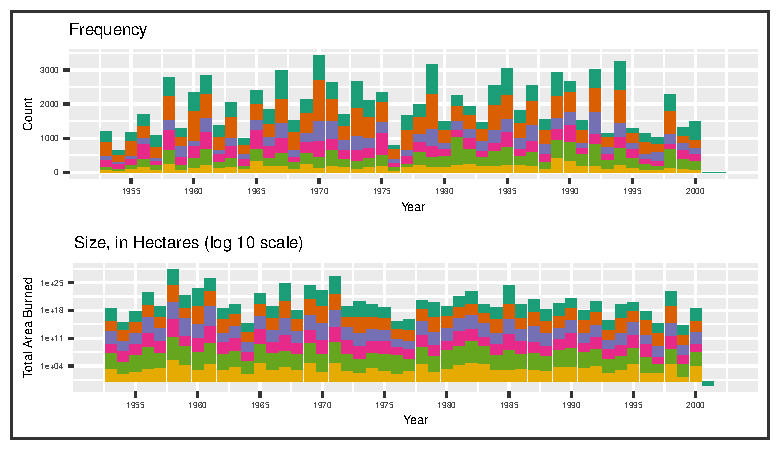
\includegraphics[width=\textwidth]{Joint_Count_Files/firezones-1.pdf}
\caption{\label{firezones}\textbf{Labelled map of zones (left) and the number
and size of fires in each zone (right).} The number of fires is equally
distributed across regions, but region 5 tends to have much larger fires
than the other regions.}
\end{figure}

For both the negative binomial model for counts and the lognormal fire
sizes, it is straightforward to include covariates in the respective
mean parameters. For fire sizes, these covariates are based on recorded
weather variables as well as variables defined by the Canadian Forest
Fire Danger Rating System \cite{wottonLightningFirePrediction2012}.
These covariates take into account the temperature, wind, amount of
fuel, moisture, and recent precipitation on the day of the fire's
ignition.

The choice of covariates for the count distribution is nontrivial. We
require a covariate that influences the number of fires over a broad
region that changes throughout the year, otherwise it would not be
descriptive of changes in expected daily numbers of fires. We downloaded
data from all weather stations in B.C.
(\url{http://climate.weather.gc.ca}) that had daily observations of
precipitation (minimum, maximum, and mean), wind (maximum gust speed),
and temperatures (minimum, maximum, and mean) between 1953 and 1995.
In total, 107 stations were included. For each day, the data were
averaged across all stations within a region. The daily average of the
measurement in a given region acts as our covariate.

Some features of our data require extra consideration. First, the
numbers of wildfires in our data have an excess of zeroes. This is overcomefg
with a hurdle model. The hurdle component in our modelling framework means that there is some probability of
seeing 0 fires in a given day and a complementary probability of a positive count.

The fire sizes in our data set are all rounded to the nearest 0.1
hectares (ha). Marginal estimates of a lognormal distribution as a
generalized linear model indicate that the mean on the log scale is less
than 0, which leads to non-ignorable rounding effects. This is further
complicated by digit preference, where multiples of 0.5 are preferred
over neighbouring values over a study period where the units of measurement changed from the imperial system to the metric system. This is yet further complicated by the fact
that fires with a size of exactly 0.1 ha make up approximately 60\% of
our data.

Fig \ref{rounding} demonstrates these coarsening issues. The recorded
distribution of fire sizes has changed drastically over time, but this
is likely an artifact of the measurements. In approximately 1975, the
fire managers switched from metric to imperial units. Since 1 hectare
\(\approx\) 0.4 acres (ac), this change can be seen in the proportion of
fires recorded as a multiple of 0.4 ha (including multiples of 0.2 ha,
which is 0.5 ac).

\begin{figure}[h!]
\centering
Fig2
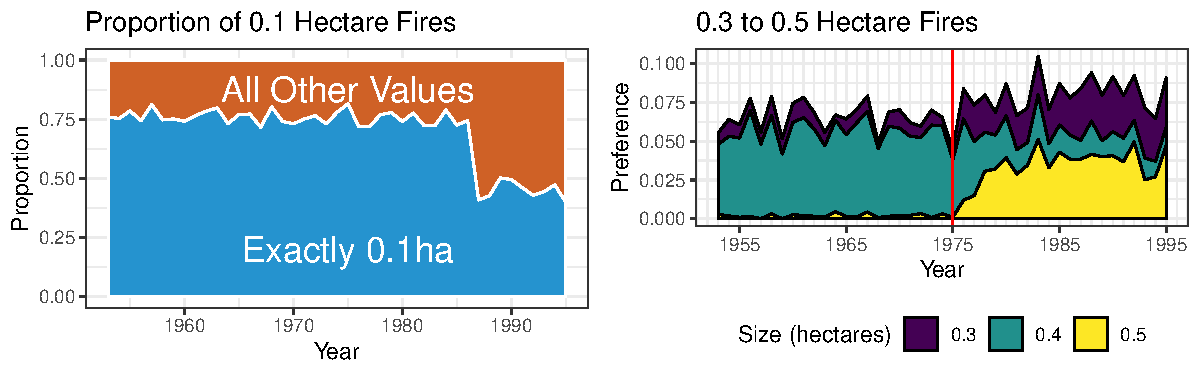
\includegraphics[width=\textwidth]{Joint_Count_Files/rounding-1.pdf}
\caption{\label{rounding}\textbf{Evidence of rounding and unit change.} Prior to
1985, 75\% of all fires were recorded as being exactly 0.1ha. The
decrease in proportion coincides with the advent of fires recorded as
0ha. In 1975, Canada switched to the metric system. This means that
fires were approximated as being 0.5ha rather tham 0.4ha (1 acre). Note
that the proportion of 0.1ha fires did not change since 1/10th of a
hectare and 1/4th of an acre are both coarsening values.}
\end{figure}

A measurement of 0.1 ha is a preferred number regardless of the unit
system (0.1 ha \(\approx\) 1/4 ac), so this did not change in the switch
from imperial to metric units. However, the number of 0.1 ha fires
decreased suddenly in 1987. Also in 1987, we see the first time where
fires were recorded as 0 ha, which was only seen a few times in 1953 to
1986. It may be the case that 0 ha fires recorded after 1987 would have
been recorded as 0.1 ha had they occurred prior to 1987.

\hypertarget{methods}{%
\section{Methods}\label{methods}}

\hypertarget{model-framework}{%
\subsection{Model Framework}\label{model-framework}}

Let \(\pi_{ir}\) represent the probability that the number of fires on
day \(i\) in region \(r\) is larger than 0, and hence \(1-\pi_{ir}\)
denotes the probability that this count is 0. To model the covariate effects, a
variety of forms of \(\pi_{ir}\) are possible; here we use logistic
regression. The number of positive counts is modeled as a negative
binomial distribution truncated at 0, with a mean that is dependent on
covariates as well as a day-specific random effect \(b_i\). Let \(N_{ir}\) be the
number of fires on day \(i\) in region \(r\). Then, we have:
\begin{align}
\begin{split}
P(N_{ir} = n|\theta^{(\pi)}, \theta^{(N)}, {Z_{ir}}^{(N)}, b_i) &= \begin{cases}
(1-\pi_{ir}) &\text{if }n=0\\
\pi_{ir}P({N_{ir}}^* = n) &\text{if }n \ge 1
\end{cases},\\
{N_{ir}}^* &\sim \text{Truncated Negative Binomial}(\lambda_{ir}, \alpha_i),\\
P({N_{ir}}^* = n|\theta^{(N)}, {Z_{ir}}^{(N)}, b_i) &= \frac{\Gamma(n + \alpha_i^{-1})}{\Gamma(\alpha_i^{-1})\Gamma(n + 1)}{\left(\frac{1}{1 + \alpha_i\lambda_{ir}}\right)}^{\alpha_i^{-1}}{\left(\frac{\alpha_i\lambda_{ir}}{1 + \alpha_i\lambda_{ir}}\right)}^{n}
\end{split}
\label{Nir}
\end{align}

\noindent where \(\theta^{(\pi)}\) refers to the vector of parameters that are
exclusive to the hurdle component of the model, \(\theta^{(N)}\) refers
to the parameters for the negative binomial model, \(Z_{ir}^{(N)}\)
refers to the covariates for the negative binomial model that were
recorded on day \(i\) in region \(r\) with coefficient vector
\(\beta^{(N)}\), \(\lambda_{ir}\) is the mean, and \(\alpha_i\) is the
dispersion of the truncated negative binomial distribution.

The parameters are modelled as follows:
\begin{align}
\begin{split}
\log(\lambda_{ir}) &= t_\lambda(i) + \lambda_r + \beta^{(N)} {Z_{ir}}^{(N)} + b_i,\\
\text{logit}(\pi_{ir}) &= t_{\pi,r}(i),\\
\log(\alpha_i) &= t_\alpha(i)
\end{split}
\label{Nirlp}
\end{align}

\noindent where \(t_\lambda(i)\), \(t_{\pi,r}(i)\), and \(t_\alpha(i)\) are
temporal trends, here modelled as P-splines with cubic basis functions \cite{langBayesianPSplines2004}
and knots defined at the deciles of the fire season. The knots were chosen under the assumption that the parameters have the same smoothness throughout the season. For further information about spline-based smoothing the interested reader is directed to the books of \cite{ramsayFunctionalDataAnalysis2006} or \cite{woodGeneralizedAdditiveModels2017} and references therein.

The sizes of the fires are modelled as lognormal. However, fire sizes
are only recorded to the first decimal place. Approximately 90\% of the
fires are less than one hectare, so this coarsening can cause dramatic
bias in the results \cite{lawEffectsMidpointImputation1992}. To account for this, we make
assumptions about the rounding behaviour. We treat all of our data as
interval censored, with intervals chosen to reflect our fire science
context. We discuss the model for the distribution of fire sizes
next, and in Section 3.2 of this paper we consider in detail how interval censoring of
the fire sizes is handled.

Let \({X_{ijr}}^*\) represent the true fire size and \(X_{ijr}\) represent
the observed fire size, then: \begin{align}
{X_{ijr}}^* &\sim \text{LogNormal}(\mu_{ijr}, \sigma^2_{r}),\\
\mu_{ijr} &= \mu_r + \beta^{(X)} Z_{ijr}^{(X)} + \gamma_rb_i
\label{Xijr1}
\end{align}

The covariates ${Z_{ijr}}^{(X)}$ were mean-centred for better convergence
properties in the Bayesian Markov Chain Monte Carlo (MCMC) algorithm
\cite{kruschkeDoingBayesianData2015}.

The shared random effect \(b_i\) is constant across the province but
different for each day of the fire season. We may model the random
effect in a variety of ways; for example with either independent
Gaussian distributions or with an autoregressive (AR) structure to account
for temporal autocorrelation: \begin{align}
\begin{split}
b_i &\sim N(0, {\sigma_b}^2)\text{, or}\\
b_0 &= 0; b_i \sim N(\phi b_{i-1}, {\sigma_b}^2)\text{, or}\\
b_{-1} &= 0;\; b_0 = 0;\; b_i \sim N(\phi_1 b_{i-1} + \phi_2 b_{i-2}, {\sigma_b}^2)
\label{ar12}
\end{split}
\end{align}

The linking parameter \(\gamma_r\) is different for each region.
This is required in the model for the size distribution to
account for the differences in scales of the two outcomes (count and size). For instance,
\(b_i = 1\) corresponds to an increase in \(e^1\) times as many fires in
the count distribution, but an increase of \(\gamma_r\) in the mean of
the size distribution. By the including this shared random effect, the
model incorporates correlation between the two outcomes. Table
\ref{interb} identifies how the shared random effect links the two
outcomes, and the effect of the correlations.

\begin{table}[h!]
\centering
\begin{tabular}{c | c c}
               & $b_i > 0$   & $b_i < 0$ \\ \hline
$\gamma_r > 0$ & Large fires, Many fires & Small, Few\\
$\gamma_r < 0$ & Small, Many & Large, Few
\end{tabular}
\caption{Interpretations of the linking parameter.}
\label{interb}
\end{table}

\hypertarget{models-for-rounded-and-heaped-fire-sizes}{%
\subsection{Models for Rounded and Heaped Fire
Sizes}\label{models-for-rounded-and-heaped-fire-sizes}}

We consider three possibilities for the true fire sizes: (M1) the data
were rounded to the nearest 0.1; (M2) most of the data were rounded to
the nearest 0.1 but some were preferentially rounded to either 0.1, 0.5,
1, 1.5, or 2; or (M3) a probabilistic mixture of these two. The
mixture model allows for a probability that it was rounded to either
level of precision at the expense of added complexity. M1 will be
referred to as rounding, M2 will be referred to as heaping, and M3
will be referred to as the mixture model.

Models M1 and M2 are achieved by treating the data as interval
censored. The same estimation algorithm is used to fit both models, but
different definitions of intervals are used.

Model M3, the mixture model, is based on
\cite{wangModelingHeapingSelf2008}. We denote the rounding regime as
\(G_{ijr}\), with regime \(G_{ijr}=1\) corresponding to rounding to the
nearest decimal place and \(G_{ijr} = 2\) corresponding to rounding to
the nearest 0.5. For example, a recorded value of 0.5 may correspond to
a true value between 0.45 to 0.55 (M1) or a true value between 0.25 and
0.75 (M2). Fires recorded as 0.1 ha are a special case and are treated
as if they are a multiple of 0.5, i.e.~their interval is 0.1 \(\pm\) 0.25,
truncated at 0.

The rounding intervals given are measured in hectares. However, as previously stated it is evident that the data collection was completed using the imperial system
prior to 1975 and the metric system after (Fig \ref{rounding}). With
the unit change came a change in digit preference. For data before 1975,
M2 relates to multiples of 1 acre; for instance, rounding to the
nearest 0.5 means nearest 0.5 ac, which is recorded in our data as
0.2 ha. Rounding to the nearest 0.1 ha remains the same regardless of the measurement units, since 0.1 ha is
approximately 0.25 ac.

Let \(X_{ijr}\) represent the observed fire size (subject to rounding
and/or coarsening), then: \begin{align}
\begin{split}
F(x) &= \int_{-\infty}^x f_{X^*}(t|\sigma_{xr}, \mu_{ijr}, b_i)dt\\
P(X_{ijr} = x|\theta^{(X)}, {Z_{ijr}}^{(X)}, b_i) &= I(G_{ijr}=1)(F(d_{12}) - F(d_{11})) + I(G_{ijr} = 2)(F(d_{22}) - F(d_{21}))\\
\text{logit}(P(G_{ijr} = 1)) &= \xi_r
\end{split}
\end{align}

\noindent where \(\underline d_1 = (d_{11}, d_{12})\) is the censoring interval
under the assumption that the data were rounded to the nearest 0.1 ha,
and \(\underline d_2\) is the censoring interval under coarsening with
indicator \(G_{ijr}\) determining which interval to use, covariates
recorded for each fire are denoted \({Z_{ijr}}^{(X)}\) with coefficient
vector \(\beta^{(X)}\), and $\xi_r$ is a constant probability of rounding within each region.

\hypertarget{estimation}{%
\subsection{Estimation}\label{estimation}}

The joint likelihood is calculated for each day as the likelihood for
the hurdle component multiplied by the product of all of the likelihoods
for each fire on that day. The conditional likelihood contributions from
each submodel are shown in Eqs (\ref{Nir}) and (\ref{Xijr1}) and
the joint likelihood is: \begin{align}\begin{split}
L_i(\theta^{(p)}, &~ \theta^{(N)}, \theta^{(X)} | N_{ir}=n, X_{ijr} = x, b_i) =\\& \prod_{r = 1}^R\left[P(N_{ir} = n|\theta^{(p)}, \theta^{(N)}, b_i)\prod_{j = 1}^{N_{ir}}P(X_{ijr} = x|\theta^{(X)}, {Z_{ijr}}^{(X)}, b_i)\right]
\label{bigLik}\end{split}\end{align}

The full likelihood is the integral of Eq (\ref{bigLik}) over all
random effects: \begin{align}
\begin{split}
L_i(\theta^{(p)}, &~ \theta^{(N)}, \theta^{(X)} | N_{ir}=n, X_{ijr} = x) =\\& \int_\mathcal{B}L_i(\theta^{(p)}, \theta^{(N)}, \theta^{(X)} | N_{ir}=n, X_{ijr} = x, b_i)d\mathbf{b}
\end{split}\end{align}

\noindent where \(\mathcal{B}\) is the joint support of the random effects.

Estimation is carried out via Markov Chain Monte Carlo (MCMC) methods
using a Gibbs sampler via the R interface to JAGS
\cite{rcoreteamLanguageEnvironmentStatistical2019,plummerJAGSProgramAnalysis2003}. To incorporate the truncated
negative binomial likelihood into JAGS, the so-called 1s trick is
employed, where the likelihood is estimated as
\(L_i(\cdot) = P(Z_{1} = 1)\) and the likelihood of \(Z_1\) is a
binomial distribution and \(Z_1\) is a vector of ones \cite{kruschkeDoingBayesianData2015}.

\hypertarget{prior-and-hyperprior-distributions}{%
\subsubsection{Prior and Hyperprior
Distributions}\label{prior-and-hyperprior-distributions}}

The prior distribution for the variance parameters of \(b_i\) and
\(X_{ijr}\) were set as uniform on the interval (0, 20), based on the
recommendations in \cite{gelmanPriorDistributionsVariance2006}. The
prior distributions for the coefficients were all chosen to be normal
with mean 0 and standard deviation 5 (giving a precision of 1/25). The
priors for the parameters in the spline terms were set according to \cite{langBayesianPSplines2004}. The parameter associated with the first basis was set as a vague normal distribution ($a_1 \sim N(\mu = 0$, $\sigma^2 = 100$)). For the remaining parameters, a prior was set for the difference, i.e. $a_j - a_{j-1} = u_j \sim N(0, 100)$.

to be multivariate normal, with
mean \(\underline 0\) and precision matrix \((A^TA)^{-1/2}\), where
\(A_{ij} = 0.1\) \(\forall\) \(i,j\). The hyperprior for the AR(1)
parameter \(\phi\) was set as uniform on the interval \([-1,1]\) to
force the AR process to be stationary.

Shared hyperpriors are used for the region-specific intercepts
\(\beta_r\) and \(\lambda_r\). In particular,
\(\beta_r \sim N(\beta_0\), precision = 1/25), where
\(\beta_0 \sim N(0,1/25)\) is the same mean for all regional parameters.
This is equivalent to a random effects model for the intercepts of each
region.

The prior distributions were also used for variable selection. This was
performed by the inclusion of an indicator variable that forces a regression
parameter to either be identically 0 or to follow a continuous posterior
distribution. The indicator \(I(\beta = 0)\) follows a Bernoulli
distribution, and the prior of the regression parameter is
\(I(\beta = 0)p(\beta)\), where \(p(\beta)\) represents the
unconstrained prior distribution. This is known as spike-and-slab
regression, as was described by
\cite{kuoVariableSelectionRegression1998}. This method was chosen based
on its simplicity, good mixing, and good separation properties as
discussed in \cite{oharaReviewBayesianVariable2009}.

\hypertarget{goodness-of-fit-and-model-comparison}{%
\subsection{Goodness of Fit and Model
Comparison}\label{goodness-of-fit-and-model-comparison}}

\hypertarget{predictions}{%
\subsubsection{Predictions}\label{predictions}}

Conditional on the random effects, predictions from the count
distribution are obtained as the expectation of the truncated negative binomial
distribution multiplied by the probability of a fire day. These marginal
predictions can be used to evaluate the root mean squared error (RMSE)
from the observed minus expected counts.

For the size distribution, predictions are not as straightforward
because the true values are rounded. A potential approach is to round
the predicted values and compare the observed minus expected number
within each bin, but this does not account for the coarsening. We
instead use a likelihood-based approach as described below.

\hypertarget{widely-applicable-information-criterion}{%
\subsubsection{Widely Applicable Information
Criterion}\label{widely-applicable-information-criterion}}

The Widely Applicable Information Criterion
(WAIC, also known as
Watanabe-Akaike Information Criterion, \cite{watanabeAsymptoticEquivalenceBayes2010,watanabeEquationsStatesSingular2010}) is used to compare models.
The calculation of the WAIC that we use is based on
\cite{gelmanUnderstandingPredictiveInformation2014a}, and our notation
in this section is identical to theirs.

The definition of WAIC is based on the log point wise predictive density
(lppd), which is a concept closely related to leave-one-out cross
validation. \begin{align*}
\text{lppd} &= \log\prod_{i=1}^np_{\text{post}}(y_i)\\
\text{computed lppd} &= \sum_{i=1}^n\log\left(\frac{1}{S}\sum_{s = 1}^Sp(y_i|\theta^s)\right)\\
\end{align*}

In the above equation, \(\theta^s\) represents the \(s\)th draw from the
posterior distribution out of $S$ total draws, based on a MCMC algorithm.
This formula calculates the average of the likelihood over all of the
draws, then sums over the log of each term.

Next, we calculate the effective number of parameters
(\(p_\text{WAIC}\)) using the second definition in
\cite{gelmanUnderstandingPredictiveInformation2014a}. This quantity is
used as a penalty for having too many unconstrained parameters.
\begin{align*}
p_\text{WAIC2} &= \sum_{i=1}^n\text{var}_\text{post}(\log(p(y_i|\theta)))\approx \text{effective number of parameters}\\
\text{computed }p_{\text{WAIC2}} &= \sum_{i=1}^nV_{s=1}^S(\log(p(y_i|\theta^s)))
\end{align*}

\noindent where the function \(V_{s=1}^S(a) = \sum_{s=1}^S(a - \bar a)^2/(S-1)\)
is the sample variance of the draws from the posterior distribution of
the parameters.

Finally, the WAIC is calculated as follows: \begin{align}
WAIC = -2(\text{lppd} - p_\text{WAIC2})
\end{align}

The WAIC was chosen because, as noted in
\cite{gelmanUnderstandingPredictiveInformation2014a} and \cite{loo2017}, it is a more
suited to the Bayesian approach in that it incorporates the entire
posterior distribution rather than a point estimate.

\hypertarget{tests-for-independence}{%
\subsection{Tests for Independence}\label{tests-for-independence}}

One of our primary goals is to quantify the dependence between the sizes
and the counts. This can be done by testing whether the linking
parameter is 0, whether the variance of the random effect is 0, or by
comparing models with and without a linking parameter.

In this paper we test whether \(\gamma_r=0\). In this case, the count
distribution retains a province-wide daily random effect and
there is no information shared between the count and size models. Hence the count
distribution is a mixed effects model. This is consistent with the findings of other authors such as
\cite{brillingerProbabilisticRiskAssessment2006} who found that a mixed effect framework was useful when modelling fire occurrence probability.

In Bayesian models, the posterior distribution is assumed to contain all
of the information about a given parameter. For our test, we can look at
whether \(\gamma_r = 0\) is a credible value. We calculate a 95\% Credible
Interval (95\%CI) and determine whether 0 is in the interval.

Other tests can be based on Bayes Factors, information criterion, or
other calculations based on the posterior distribution as discussed in
the Appendix. We note that the CI method is by far the simplest and
performs just as well as the other tests with regards to the binary
decisions in our simulations. Another advantage of this framework is
that we are able to test for dependence within a single region.
Tests based on model comparisons are not easily amenable to such
situations.

\hypertarget{results}{%
\section{Results}\label{results}}

Models were fit separately to different years and for each of the
two causes. For consistency across years, the optimal model was the one
with the lowest WAIC for the most amount of years. For the lightning
fires, this is a model with coarsening (M2), a spline for the hurdle
component that is constant across the province, and an AR1 structure.
The best models for person-caused fires also include M2 and an AR(1)
structure, but had different spline terms for each region.

Fig \ref{gammaltg} and Fig \ref{gammaper} show the estimates for the
linking parameter for each year along with a 95\% CI for lightning- and person-caused fires, respectively. The points and intervals are coloured based on whether they
are entirely above 0, entirely below 0, or contain 0.

\begin{figure}[h!]
\centering
Fig3
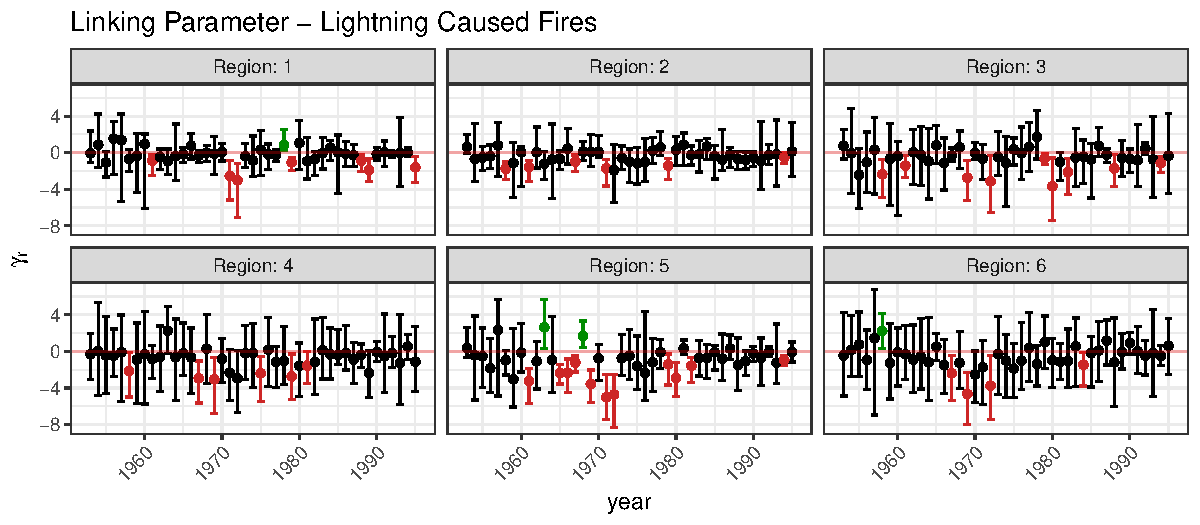
\includegraphics[width=\textwidth]{Joint_Count_Files/gammaltg-1.pdf}
\caption{\label{gammaltg}\textbf{Posterior median estimates and 90\% Credible
Intervals for the linking parameter in the model for lightning-caused
fires.} There are very few years where the credible interval was entirely
above 0, but several where it was below. This indicates that the size and
count of lightning-caused fires often a negative association.
Days with fewer fires had larger fires, and days with more fires had
smaller fires.}
\end{figure}

\begin{figure}[h!]
\centering
Fig4
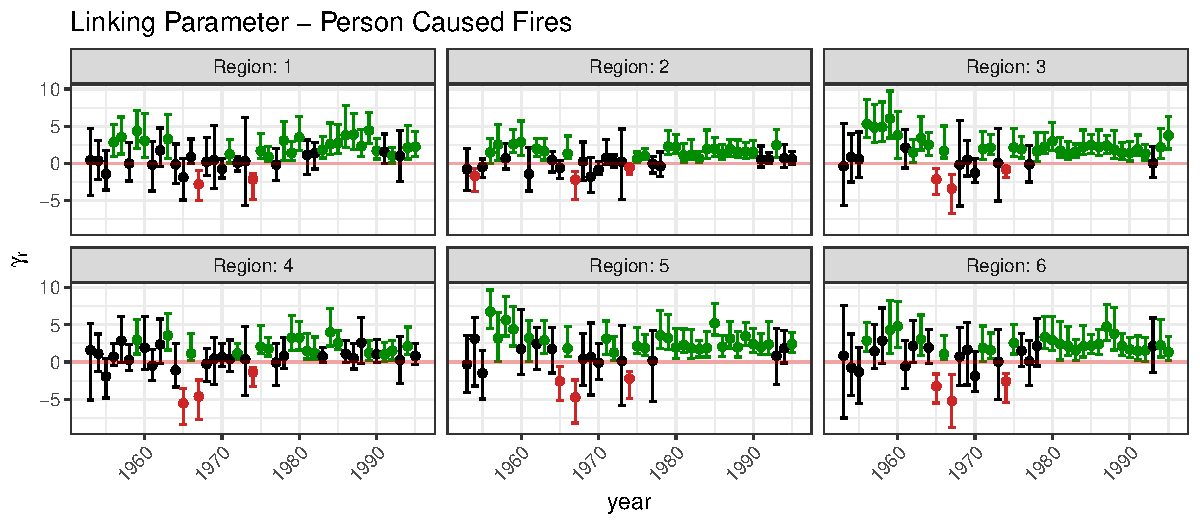
\includegraphics[width=\textwidth]{Joint_Count_Files/gammaper-1.pdf}
\caption{\label{gammaper}\textbf{Posterior median estimates and 90\% Credible
Intervals for the linking parameter in the model for person-caused
fires.} In contrast to lightning-caused fires, person-caused fires tend
to have positive association.}
\end{figure}

For lightning-caused fires, the credible intervals that do not contain 0
are almost all negative, indicating that days with many fires tend to
have smaller fires, and days with few fires tend to have larger fires.
If there are many lightning-caused fires, then we expect that there are
many days with lightning strikes and thus many rainy days. Multiple
rainy days throughout the year would contribute to there being fewer
fires. Since we included covariates that already account for the amount
of rain on a single day, our model is capturing dependence on a larger
time scale.

In contrast to lightning-caused fires, person-caused fires tend to have
a positive association. If there are many person-caused fires, then this
is likely due to an increase in human activity. This might be due to
increased recreational activity or increased forestry activity, both of
which would be associated with a lack of rain. Again our inclusion of
weather covariates indicates that this observed dependence is either not
based on the weather or occurs on a broader time scale.

Fig \ref{hypers} shows the hyperparameters and their 95\% CIs for both
causes. These plots do not show any clear trend over time in the mean of
either outcome. The values on the y-axis indicate that lightning-caused
fires tend to be larger but there are fewer of them.

\begin{figure}[h!]
\centering
Fig5
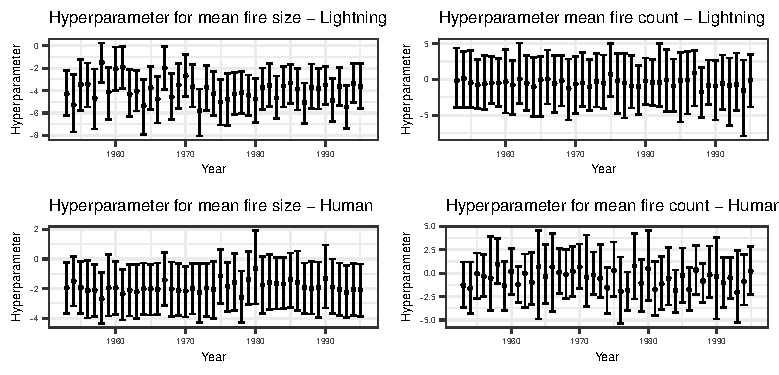
\includegraphics[width=\textwidth]{Joint_Count_Files/hypers-1.pdf}
\caption{\label{hypers}\textbf{Hyperparameters for the mean of the size and
count.} By the construction of the model, the regional parameters are
deviations from these values, with the hyperparameters representing the
mean over all regions. All of these parameters are on the log scale.}
\end{figure}

Spatial and temporal correlations in the linking parameters are
displayed in Fig \ref{spatialcor}. These correlations are calculated
from the medians of the posterior distributions of the linking parameter. These correlations do not indicate any
pattern over time for the linking parameter.

\begin{figure}[h!]
\centering
Fig6
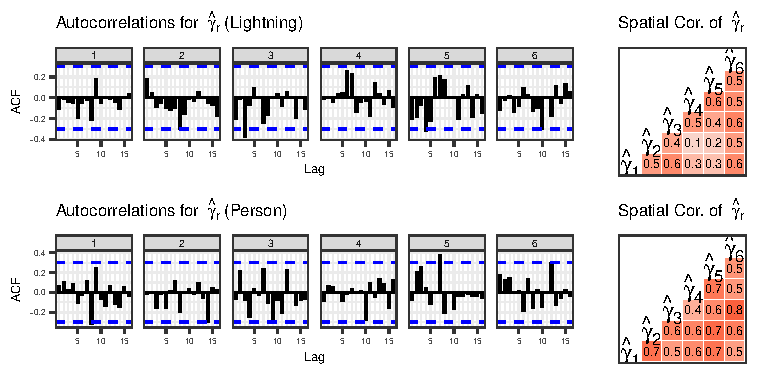
\includegraphics[width=\textwidth]{Joint_Count_Files/spatialcor-1.pdf}
\caption{\label{spatialcor}\textbf{Correlation of the estimated linking
parameter across space and time.} The linking parameter in one year does
not appear to predict the linking parameter in the next year. The
linking parameter for lightning-caused fires is correlated for regions 1
and 2 (which are both interior from the coast and with similar forest
cover) and regions 4 and 5 (which have no clear similarities). There is
province-wide correlation among the linking parameters for person-caused
fires.}
\end{figure}

Estimated linking parameters for lightning-caused fires in regions 1 and
2 and regions 4 and 5 have the strongest correlations. Regions 1 and 2
are neighbours in a mountainous inland region, so their similarity is
not surprising. Region 4 is a coastal region including Vancouver Island,
while region 5 is a northern region to the east of the mountains.

For person-caused fires, the point estimates of \(\gamma_r\) in all of
the regions appear to be strongly correlated. This indicates that if
fire managers observe many large fires (or few small fires) in one
region, they can expect something similar in another region. This only
applies to human-caused fires, which may mean that this dependence is
capturing broad weather trends or long weekends that lead to more (or less) human
activity which has the possibility of igniting fires. This might manifest
as increased recreational use or increased industrial activity, such as logging.

Fig \ref{sigestl} and Fig \ref{sigestp} show the estimates of the
variance parameters for lightning- and person-caused fires,
respectively. Again, there is no clear pattern over time for lognormal
variance ${\sigma_r}^2$ in the years in this study. However, the variance of the random
effect ${\sigma_b}^2$ appears to be decreasing and the autoregressive parameter appears
to be increasing. Since the random effect is shared between the models,
this means that the variance of both models decreased, indicating that
both the count and size of fires are less variable day-to-day. The
increase in the autoregressive parameter $\phi$ also supports this conclusion.

\begin{figure}[h!]
\centering
Fig7
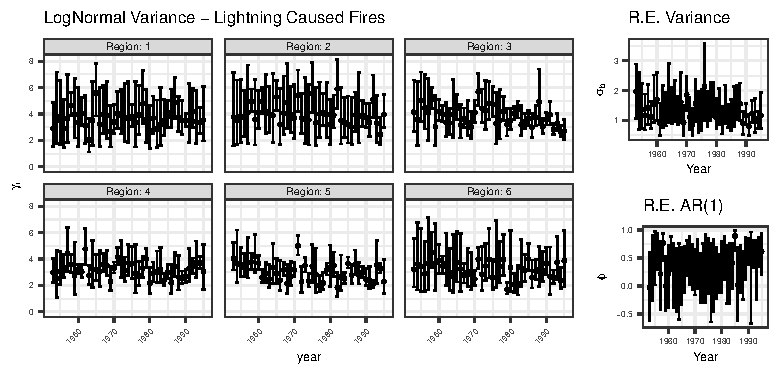
\includegraphics[width=\textwidth]{Joint_Count_Files/sigestl-1.pdf}
\caption{\label{sigestl}\textbf{The variance parameters for lightning-caused
fires.} there is no apparent trend over time, except perhaps a slight
decrease in region 5 and in the random effect variance, with an increase
in the AR(1) parameter. The AR(1) parameter is constrained to be in the
interval {[}-1,1{]}.}
\end{figure}

\begin{figure}[h!]
\centering
Fig8
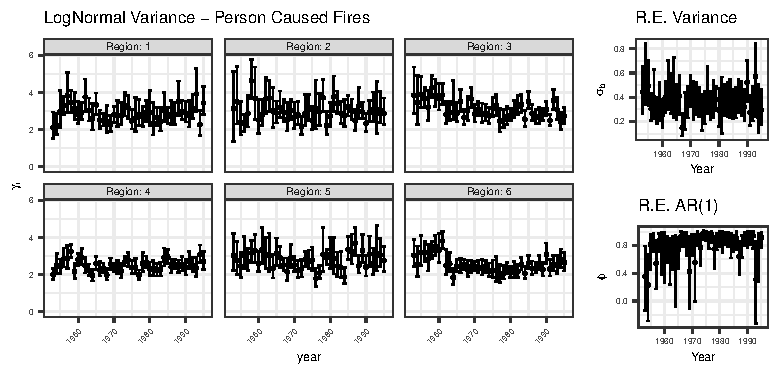
\includegraphics[width=\textwidth]{Joint_Count_Files/sigestp-1.pdf}
\caption{\label{sigestp}\textbf{Variance parameters for person-caused fires.}
Again, there is a slight decrease in the estimates for region 5 and
\(\sigma_b\) with an increase in the AR(1) parameter.}
\end{figure}

Finally, note that the prior distribution for the autoregressive
parameters is restricted to {[}-1, 1{]}, meaning that the AR model is
constrained to be stationary. The bottom right plot in Fig
\ref{sigestp} (the variance plots for person-caused fires) demonstrates
that this constraint may be too constrictive, and that the random effect
is not stationary within each year.

\hypertarget{conclusions-and-discussion}{%
\section{Conclusions and Discussion}\label{conclusions-and-discussion}}

We have introduced a model that allows for dependence between a zero-heavy count distribution and the summands of those counts. This was accomplished
with a shared random effect, which is on the scale of the log of the
number of fires and has a linking parameter in the size
distribution. Such a framework could be employed in other contexts for
jointly modelling the frequency and severity of events, such as
insurance claims, hospital stays, or the number of herds along with the herd size.

One of the consequences of our model formulation is that the linking parameter provides a convenient foundation for a test of
independence. For our data, the tests for independence concluded that
there is indeed a form of independence between the number and the size
of forest fires. The independence between these two is different depending
on the cause of the fires. Lightning-caused fires tend to have negative
dependence, whereas person-caused fires have positive dependence.

From the observed differences in direction of dependence among lightning- and person-caused fires, it appears that the dependence
between size and count is driven by covariates that are either not
observed or not observable. It is also possible that other physical
properties are driving the dependence. Also note that person-caused
fires are, on average, smaller than lightning-caused fires, and the
dependence must be interpreted carefully.

We did not find any systematic changes in the parameter estimates over
time. However, the data set presented in this paper only includes data
up until 1995. Another data set is available with data up to 2015, but
these data do not include covariate information. Analysis of the second
data set has found several systematic patterns that are more prominent
in 1995-2015. In particular, the lognormal variance parameters
\(\sigma_r\) decrease while the random effect variance increases,
indicating that the variance is better explained by the joint framework
than the individual models alone. Neither data set includes 2017 or
2018, which were years with a large number of very large fires.

When $\gamma = 0$ the random effects term in the size distribution vanishes. This does not imply that there is no excess variability in the size distribution; it implies that any possible excess variability in the sizes is different from the excess variability in the counts. For models where $\gamma = 0$ it is still worthwhile to investigate a different day-specific random effect in each distribution. Incorporating this second random effect may or may not explain the observed pattern in the variance parameters; future work should investigate this.

A potential limitation to this study is that the linking parameter was
constant over each year. We have investigated the use of spline terms
for the linking parameter over the course of the fire season. According
to the WAIC for each year, this adds too much complexity to the models.
However, a future study might involve some other non-constant linking
parameter, such as a piece-wise constant with carefully chosen time knots.

Another potential limitation is the size of the regions that we used. We
assumed that they were approximately homogeneous, but regions 5 and 6
are much larger than the other regions (they are each approximately the size of the United Kingdon), so it is unlikely
that these regions are truly homogeneous. The regions were chosen
primarily for their homogeneity with respect to fire management efforts,
but it may be useful to explore finer spatial partitions of the study region in future work, such as partitioning according to ecoregions (e.g., \cite{ecologicalstratificationworkinggroupcanadaNationalEcologicalFramework1996}). The definition of ecoregion should be chosen based on domain
knowledge of wildland fire ecology.

Due to the spatial and temporal correlation found in this model, it may
be useful to fire managers to have a version of this model that updates
throughout the fire season to provide estimates of what type of year it
is: positive dependence, negative dependence, or neutral. The AR
structure in the random effect allows for prediction. If the linking
parameter is negative and the random effects have been positive, fire
managers could expect fewer fires but also be prepared for a large fire.
To provide this to fire managers, the model would need to be deployed on
a system that is easily accessed and understood.

\hypertarget{acknowledgements}{%
\section{Acknowledgements}\label{acknowledgements}}

%We acknowledge the generous support of the Natural Sciences and
%Engineering Research Council of Canada, the Canadian Statistical
%Sciences Institute, and the Institute for Catastrophic Loss Reduction.
We wish to thank Steve Taylor of the Pacific Forestry Centre in
British Columbia for providing the data and Da Zhong Xi for
pre-processing the data.

All analyses were done using the R statistical software language
\cite{rcoreteamLanguageEnvironmentStatistical2019}. The R packages
\texttt{dplyr} \cite{Wickham}, \texttt{tidyr} \cite{Wickham2018},
\texttt{ggplot2} \cite{Wickham2016}, \texttt{ggmap}, \cite{Kahle2013},
\texttt{spatstat} \cite{baddeleySpatstatPackageAnalyzing2005},
\texttt{sp} \cite{pebesmaClassesMethodsSpatial2005}, \texttt{raster}
\cite{hijmansRasterGeographicData2019}, and \texttt{JAGS}
\cite{plummerJAGSProgramAnalysis2003} were used extensively in this
research.

\hypertarget{appendix-b-model-selection-power-study}{%
\section{Appendix A: Model Selection ``Power
Study''}\label{appendix-b-model-selection-power-study}}


\hypertarget{simulation-setup}{%
\subsection{Simulation Setup}\label{simulation-setup}}

In this appendix, we simulate from a simpler version of our model with
varying degrees of separability and test which methods would lead to the
correct conclusion. The simpler version of the model includes a single
region and uses a simple negative binomial distribution for the count
with no hurdle component and a constant mean and dispersion. The
``true'' sizes are lognormally distributed with a constant mean and
variance. \begin{align*}
N_i &\sim \text{NegBinom}(\lambda_i = \exp(\lambda + b_i), \alpha)\text{;\; }i=1...215\\
{X_{ij}}^* &\sim \text{LogNormal}(\mu_i = \mu + \gamma b_i, \sigma_x)\text{;\; }j = 1...N_i\\
X_{ij} &= \begin{cases}
\text{round}({X_{ij}}^*, g_1) & \text{w.p. }p_r\\
\text{round}({X_{ij}}^*, g_2) & \text{w.p. }1-p_r
\end{cases}\\
b_i &\sim N(0, \sigma_b)
\end{align*}

We considered parameters based on our estimates above, with
\(\lambda = (-1,~-0.5,~0)\), \(\sigma_b = (0.25,~0.5,~1)\),
\(\sigma_x = 1\), and \(\alpha = 0.8\). Our simulated data were rounded
according to our assumed data generating process for our data, with a certain proportion of fires being
rounded to the nearest 0.1 (represented by round(\({X_{ij}}^*, g_1\))) or
to 0, 0.1, 0.5, 1, 1.5, or 2 (\(g_2\)). To determine the power, we
looked at values of \(\gamma\) from 0 to 1. We simulated 100 data sets
from each combination of parameters.

\hypertarget{bayesian-model-selection}{%
\subsection{Bayesian Model Selection}\label{bayesian-model-selection}}

The most popular method of model selection is the Bayes Factor (BF),
which is similar to the likelihood ratio in frequentist statistics. The
BF is calculated as the ratio of the marginal likelihoods: \begin{align}
BF_{01} = \frac{p(\mathbf y | \mathcal{M}_0)}{p(\mathbf y | \mathcal{M}_1)} =
\frac{\int_{\Theta_0} p(\mathbf y | \theta_0, \mathcal{M} _0)\pi_0(\theta_0)d\theta_0}{\int_{\Theta_1} p(\mathbf y | \theta_1, \mathcal{M} _1)\pi_1(\theta_1)d\theta_1}
\label{BF}
\end{align}

In Eq (\ref{BF}), \(\pi_0(\theta_0)\) and \(\pi_1(\theta_1)\) are
the prior distributions for parameter vectors \(\theta_0\) and
\(\theta_1\), respectively. The BF does not rely on the posterior
estimates of the data.

The BF does not exist in closed form for our model. There are several
approximations to the marginal likelihoods that we investigated. A
common approximation is the Harmonic Mean, which is shown in Eq
(\ref{HM}). This approximation relies on posterior samples of the
likelihood rather than prior samples. The harmonic mean estimate is
criticised as having an infinite variance.
\begin{align}
\int_{\Theta_1} p(\mathbf y | \theta)\pi(\theta)d\theta = E_{\pi(\theta)}[p(\mathbf y | \theta)] \approx {\left[\frac{1}{S}\sum_{s = 1}^S\frac{1}{p(\mathbf y | \theta^{(s)})}\right]}^{-1} = HM_{01}
\label{HM}
\end{align}

In Eq (\ref{HM}), \(S\) represents the number of samples from the
posterior distribution and \(\theta^{(s)}\) is the \(s\)th sample of the
parameter vector \(\theta\) from a Gibbs sampling algorithm.

The harmonic mean is used to avoid numerical instability. The values of
the likelihood tend to be too small for a computer to represent, whereas
the inverse is not. If the numbers are not too small, one can simply
look at the mean of the posterior samples of the likelihood. If the numbers are too large, the logarithm of the likelihood can be used.

In applying Eq (\ref{HM}), it was found that the likelihood values
were still too small. To deal with this, we exploit the fact that the BF
is a ratio. Adding a constant to each of log likelihood contributions
does not change the ratio, so we subract the largest log likelihood
value.
\begin{align}
p(\mathbf y |\hat\theta_j) &= \prod_{i = 1}^N(p(y_i|\hat\theta_j))\text{;\; }j = 1,2\\
a &= \max\{\max_i[\log(p(y_i | \hat\theta_0))], \max_i[\log(p( y_i | \hat\theta_1))]\}\\
\frac{E(\sum_{i=1}^N\log(p(y_i|\hat\theta_0) - a))}{E(\sum_{i=1}^N\log(p(y_i|\hat\theta_1) - a))} &=\frac{\exp(a^N)}{\exp(a^N)} BF_{01} = BF_{01}
\end{align}

This identity greatly improved the stability of the Bayes Factors
computation.

Another estimate is the Naive Bayes Estimator. This is the estimator
that arises naturally from the first two expressions in Eq (\ref{HM}), where we are interested
in the expectation of the likelihood with respect to the prior
distributions. The primary issue with this estimate is numerical
stability. The draws from the prior distribution will often be in areas
of low density for the likelihood, so there will be many values that are
indistinguishable from 0. We included this estimate in our analysis, but
the numerical instability is apparent in the results.

The final estimate of the BF that we consider is known as the
Savage-Dickey Density Ratio (SDDR). The SDDR is only applicable in tests
where \(\mathcal M_0\) is a point density and \(\mathcal M_1\) is a
distribution (e.g.~\(\gamma = 0\) versus \(\gamma \sim \pi(\gamma)\)).
The SDDR for testing a parameter equal to 0 is calculated as follows:
\begin{align}
SDDR_{01} = \frac{\pi(0)}{\pi(\hat\theta)|_{\hat\theta = 0}}
\end{align}

This is simply the ratio of the value of the prior distribution at 0
divided by the value of the posterior distribution at 0.

For all of the BF estimates, we convert the Bayes Factor into a binary decision by treating any BF larger than 3 as evidence against $M_0$. This value was chosen based on
hueristic guidelines from \cite{jeffreysTheoryProbability1998}, who
define a BF between 3 and 10 to be ``moderate evidence.''

Other model selection methods that do not invlolve Bayes Factors are
also investigated. The Bayesian framework allows for probabilistic
assessments of the parameters in the model, so several frameworks for
testing point-Null hypotheses have been proposed. We employ two in
particular, as implemented in the \texttt{bayestestR} R package
(\cite{makowskiUnderstandDescribeBayesian2019}).

The first is the Probability of Direction (pd), introduced in
\cite{makowskiIndicesEffectExistence2019}. This is defined as the
integral of the posterior distribution from 0 to either positive or
negative \(\infty\), depending on the sign of the median of the
posterior.

The second is the Region of Practical Equivalence (ROPE) test. This test
sets up a region around the null value (0 in this case) that would be
considered ``practically equivalent,'' i.e.~close enough to 0 to be
indistinguishable. Usually, this region is \(0\) plus or minus one standard
deviation of the posterior distribution. The ROPE test reports the
proportion of the Highest Density Interval that lines within the ROPE.

In both tests, a cutoff point must be chosen. To be consistent with
previous studies, we use a 5\% cutoff value. This is approximately
equivalent to a p-value. We note that there is no equivalence between
p-values and Bayes Factors (see,
e.g.~\cite{lindleyStatisticalParadox1957}).

Similar to \cite{luoPerformancesLOOWAIC2017}, we also employ a binary
test based on the WAIC. For this study, we simply compare the difference
in WAIC between the full model and a model with \(\gamma\) constrained
to be 0. Since WAIC is fully Bayesian, the full posterior distributions
of the WAIC in each model could be compared. However, we have not
encountered a principled approach to such a comparison, so we simply
look at the difference in WAIC.

The variable selection method that we employed for the covariates can
also be applied as a fully Bayesian test of a point null hypothesis. The
posterior can be constrained to 0 with some probability, and this
probability can be a parameter in the model. The probability that the
posterior is identically 0 works as a hypothesis test. Again, we use the
5\% cutoff.

The final test that we consider is the one that we used in this paper.
The posterior distribution contains all of the information about the
parameter, so simply constructing a credible interval and checking
whether 0 is in that interval should be sufficient. Again, we use a 5\%
cutoff as a binary test.

\hypertarget{power-study-results}{%
\subsection{Power Study Results}\label{power-study-results}}

The results of this power study are shown in Fig \ref{powers}.
Unsurprisingly, all of the methods performed better when there was more
data available (i.e.~with larger \(\lambda\), there are more observed $X_{ij}s$). The tests also had more
power when \(\sigma_b\) was larger.
Low values of $\sigma_b$ also represent a small effect size which explains the low power in all of the tests.

\begin{figure}[h!]
\centering
Fig9
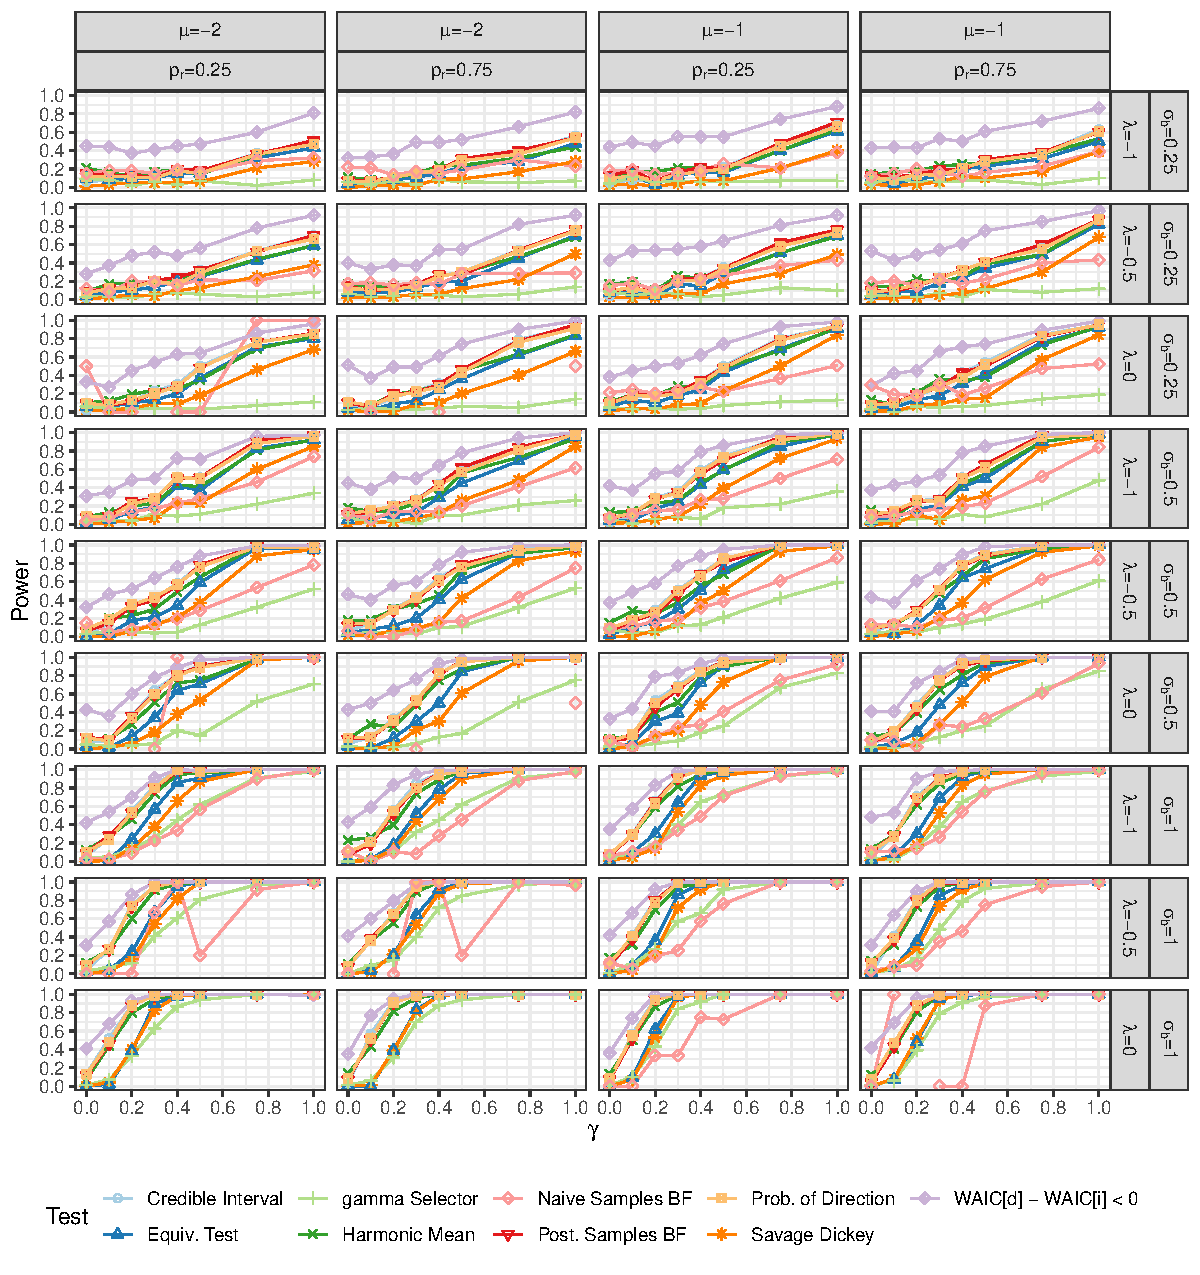
\includegraphics[width=\textwidth]{Joint_Count_Files/powers-1.pdf}
\caption{\label{powers}\textbf{Results of the power study.} The credible interval
test and the Bayes factors that relied on posterior samples performed
the best overall. Simply looking at whether the WAIC is smaller has high
power at the expense of high type 1 error. The Savage Dickey
representation of the BF might have higher power with better prior
distributions. Using the variable selection method on \(\gamma\) has
very low power, likely because \(\gamma\) is the coefficient of a latent
variable rather than an observed covariate. The equivalence test and
probability of direction have slightly lower power than simply checking
the credible interval.}
\end{figure}

The estimates of the BF based on posterior draws performed quite well,
and the credible interval and pd tests were approximately equivalent.
Since the credible interval test is easily calculated, this test is
preferred.

The pd is also easy to calculate and provide a one-sided test where the
direction is chosen based the posterior. In the frequentist framework,
this concept would be troublesome as it is choosing the direction of the
test based on which one gives a smaller p-value. However, the Bayesian
posterior distribution does not have the same interpretation and thus
avoids the issue of testing multiple hypotheses in search of a significant result (sometimes referred to as p-hacking).

As is expected, the power of the WAIC test is approximately 50\% when
\(\gamma\) is constrained to 0. In light of this, the power results are
not as impressive as they seem.

The numerical instability of the BF estimate based on prior samples is
obvious. In some cases, there were no BF estimates that had non-zero
marginal probabilities, and so there is no estimate of the power.

The SDDR has the lowest power out of all of the Bayes Factor estimates.
This is likely because the SDDR is very sensitive to the choice of
prior.

The variable selection method also performed quite poorly. This is
likely because of the extra variation introduced by the latent variable
which would not be present in observed covariates.
\nolinenumbers

% Either type in your references using
% \begin{thebibliography}{}
% \bibitem{}
% Text
% \end{thebibliography}
%
% or
%
% Compile your BiBTeX database using our plos2015.bst
% style file and paste the contents of your .bbl file
% here. See http://journals.plos.org/plosone/s/latex for
% step-by-step instructions.
%


%\bibliography{All}
\begin{thebibliography}{10}

\bibitem{taylorWildfirePredictionInform2013}
Taylor SW, Woolford DG, Dean CB, Martell DL.
\newblock Wildfire {{Prediction}} to {{Inform Management}}: {{Statistical
  Science Challenges}}.
\newblock Statistical Science. 2013;28(4,):586--615.

\bibitem{kayAreLightningFires2007}
Kay CE.
\newblock Are Lightning Fires Unnatural? {{A}} Comparison of Aboriginal and
  Lightning Ignition Rates in the {{United States}}.
\newblock In: Fire in {{Grasslandand Shrubland Ecosystems}}. {Tallahassee, FL};
  2007.

\bibitem{wulfsohnJointModelSurvival1997a}
Wulfsohn MS, Tsiatis AA.
\newblock A {{Joint Model}} for {{Survival}} and {{Longitudinal Data Measured}}
  with {{Error}}.
\newblock Biometrics. 1997;53(1):330.
\newblock doi:{10.2307/2533118}.

\bibitem{dunsonBayesianLatentVariable2000}
Dunson DB.
\newblock Bayesian {{Latent Variable Models}} for {{Clustered Mixed Outcomes}}.
\newblock Journal of the Royal Statistical Society Series B (Statistical
  Methodology). 2000;62(2):355--366.

\bibitem{juarez-colungaJointModelingZeroinflated2017}
Juarez-Colunga E, Silva GL, Dean CB.
\newblock Joint Modeling of Zero-Inflated Panel Count and Severity Outcomes.
\newblock Biometrics. 2017;73(4):1413--1423.
\newblock doi:{10.1111/biom.12691}.

\bibitem{martellLogisticModelPredicting}
Martell DL, Otukol S, Stocks BJ.
\newblock A Logistic Model for Predicting Daily People-Caused Forest Fire
  Occurence in {{Ontario}}.
\newblock Canadian Journal of Forest Research. 1987;17:394--401.

\bibitem{cunninghamStochasticModelOccurence}
Cunningham AA, Martell DL.
\newblock A {{Stochastic Model}} for the {{Occurence}} of {{Man}}-Caused
  {{Forest Fires}}.Pdf.
\newblock Canadian Journal of Forest Research. 1973;3:282--287.

\bibitem{plucinskiPredictingNumberDaily2014}
Plucinski M, McCaw WL, Gould JS, Wotton BM.
\newblock Predicting the Number of Daily Human-Caused Bushfires to Assist
  Suppression Planning in South-West {{Western Australia}}.
  2014;doi:{10.1071/WFI3090}.

\bibitem{josephSpatiotemporalPredictionWildfire2019}
Joseph MB, Rossi MW, Mietkiewicz NP, Mahood AL, Cattau ME, St~Denis LA, et~al.
\newblock Spatiotemporal Prediction of Wildfire Size Extremes with {{Bayesian}}
  Finite Sample Maxima.
\newblock Ecological Applications. 2019;0(0):e01898.
\newblock doi:{10.1002/eap.1898}.

\bibitem{brillingerRiskAssessmentForest2003}
Brillinger DR, Preisler HK, Benoit JW.
\newblock Risk {{Assessment}}: {{A Forest Fire Example}}.
\newblock Lecture Notes-Monograph Series. 2003;40:177--196.

\bibitem{preislerProbabilityBasedModels2004}
Preisler HK, Brillinger DR, Burgan RE, Benoit JW.
\newblock Probability Based Models for Estimation of Wildfire Risk.
\newblock International Journal of Wildland Fire. 2004;13(2):133.
\newblock doi:{10.1071/WF02061}.

\bibitem{vilarModelPredictingHumancaused2010}
Vilar L, Woolford DG, Martell DL, Mart{\'i}n MP.
\newblock A Model for Predicting Human-Caused Wildfire Occurrence in the Region
  of {{Madrid}}, {{Spain}}.
\newblock International Journal of Wildland Fire. 2010;19(3):325.
\newblock doi:{10.1071/WF09030}.

\bibitem{woolfordSpatiotemporalModelPeopleCaused2011}
Woolford DG, Bellhouse DR, Braun WJ, Dean CB, Martell DL, Sun J.
\newblock A {{Spatio}}-Temporal {{Model}} for {{People}}-{{Caused Forest Fire
  Occurrence}} in the {{Romeo Malette Forest}}.
\newblock Journal of Environmental Statistics. 2011;2(1):26.

\bibitem{woolfordSitespecificSeasonalBaselines2009}
Woolford DG, Braun WJ.
\newblock Site-Specific Seasonal Baselines for Fire Risk in {{Ontario}}.
\newblock Geomatica. 2009;63(4).

\bibitem{serraSpatiotemporalLogGaussianCox2014}
Serra L, Saez M, Mateu J, Varga D, Juan P, {D{\'i}az-{\'A}valos} C, et~al.
\newblock Spatio-Temporal Log-{{Gaussian Cox}} Processes for Modelling Wildfire
  Occurrence: The Case of {{Catalonia}}, 1994\textendash{}2008.
\newblock Environmental and Ecological Statistics. 2014;21(3):531--563.
\newblock doi:{10.1007/s10651-013-0267-y}.

\bibitem{schoenbergDistributionWildfireSizes2003}
Schoenberg FP, Peng R, Woods J.
\newblock On the Distribution of Wildfire Sizes.
\newblock Environmetrics. 2003;14(6):583--592.
\newblock doi:{10.1002/env.605}.

\bibitem{cummingParametricModelFiresize2001}
Cumming SG.
\newblock A Parametric Model of the Fire-Size Distribution.
\newblock Canadian Journal of Forest Research. 2001;31(8):1297--1303.
\newblock doi:{10.1139/x01-032}.

\bibitem{malamudForestFiresExample1998}
Malamud BD, Morein G, Turcotte DL.
\newblock Forest {{Fires}}: {{An Example}} of {{Self}}-{{Organized Critical
  Behavior}}.
\newblock Science. 1998;281(5384):1840--1842.
\newblock doi:{10.1126/science.281.5384.1840}.

\bibitem{podurCompoundPoissonModel2009}
Podur JJ, Martell DL, Stanford D.
\newblock A Compound Poisson Model for the Annual Area Burned by Forest Fires
  in the Province of {{Ontario}}.
\newblock Environmetrics. 2009; p. n/a--n/a.
\newblock doi:{10.1002/env.996}.

\bibitem{reedPowerlawBehaviourParametric2002}
Reed WJ, McKelvey KS.
\newblock Power-Law Behaviour and Parametric Models for the Size-Distribution
  of Forest Fires.
\newblock Ecological Modelling. 2002;150(3):239--254.
\newblock doi:{10.1016/S0304-3800(01)00483-5}.

\bibitem{paikschoenbergTestingSeparabilitySpatialTemporal2004}
Schoenberg FP.
\newblock Testing {{Separability}} in {{Spatial}}-{{Temporal Marked Point
  Processes}}.
\newblock Biometrics. 2004;60(2):471--481.
\newblock doi:{10.1111/j.0006-341X.2004.00192.x}.

\bibitem{vazquezPatternsLightningPeopleCaused1998}
Vazquez A, Moreno JM.
\newblock Patterns of {{Lightning}}-, and {{People}}-{{Caused Fires}} in
  {{Peninsular Spain}}.
\newblock International Journal of Wildland Fire. 1998;8(2):103--115.
\newblock doi:{10.1071/wf9980103}.

\bibitem{burkeHistoricFiresCentral2014}
Burke CJ.
\newblock {Historic fires in the central Western Cascades, Oregon}.
\newblock Oregon State University; 2014.

\bibitem{keeleyDistributionLightningManCaused1982}
Keeley JE.
\newblock Distribution of {{Lightning}}- and {{Man}}-{{Caused Wildfires}} in
  {{California}}.
\newblock {Berkeley, CA}: {U.S. Department of Agriculture}; 1982.

\bibitem{keenshawSituationalInfluencesAcceptable2004}
Keenshaw K, Vaske JJ, Bright AD, Absher JD.
\newblock Situational {{Influences}} of {{Acceptable Wildland Fire Management
  Actions}}.
\newblock Society \& Natural Resources. 2004;17(6):477--489.
\newblock doi:{10.1080/08941920490452427}.

\bibitem{podurSpatialPatternsLightningcaused2003}
Podur J, Martell DL, Csillag F.
\newblock Spatial Patterns of Lightning-Caused Forest Fires in {{Ontario}},
  1976\textendash{}1998.
\newblock Ecological Modelling. 2003;164(1):1--20.
\newblock doi:{10.1016/S0304-3800(02)00386-1}.

\bibitem{wottonLightningFireOccurrence2005}
Wotton BM, Martell DL.
\newblock A Lightning Fire Occurrence Model for {{Ontario}}.
\newblock Canadian Journal of Forest Research. 2005;35(6):1389--1401.
\newblock doi:{10.1139/x05-071}.

\bibitem{wottonLightningFirePrediction2012}
Wotton BM.
\newblock A Lightning Fire Prediction System. 2012;.

\bibitem{vanwagnerDevelopmentStructureCanadian1987a}
Van~Wagner CE.
\newblock Development and Structure of the {{Canadian Forest Fire Weather Index
  System}}. vol.~35; 1987.

\bibitem{wottonInterpretingUsingOutputs2009}
Wotton M.
\newblock Interpreting and Using Outputs from the {{Canadian Forest Fire Danger
  Rating System}} in Research Applications.
\newblock Environmental and Ecological Statistics. 2009;16:107--131.
\newblock doi:{10.1007/s10651-007-0084-2}.

\bibitem{albert-greenMethodologyInvestigatingTrends2013}
{Albert-Green} A, Dean CB, Martell DL, Woolford DG.
\newblock A Methodology for Investigating Trends in Changes in the Timing of
  the Fire Season with Applications to Lightning-Caused Forest Fires in
  {{Alberta}} and {{Ontario}}, {{Canada}}.
\newblock Canadian Journal of Forest Research. 2013;43(1):39--45.
\newblock doi:{10.1139/cjfr-2011-0432}.

\bibitem{hanesFireregimeChangesCanada2019}
Hanes CC, Wang X, Jain P, Parisien MA, Little JM, Flannigan MD.
\newblock Fire-Regime Changes in {{Canada}} over the Last Half Century.
  2019;49:256--269.
\newblock doi:{10.1139/cjfr-2018-0293}.

\bibitem{langBayesianPSplines2004}
Lang S, Brezger A.
\newblock Bayesian {{P}}-{{Splines}}.
\newblock Journal of Computational and Graphical Statistics.
  2004;13(1):183--212.
\newblock doi:{10.1198/1061860043010}.

\bibitem{ramsayFunctionalDataAnalysis2006}
Ramsay J, Silverman BW.
\newblock Functional {{Data Analysis}}.
\newblock {Springer Science \& Business Media}; 2006.

\bibitem{woodGeneralizedAdditiveModels2017}
Wood SN.
\newblock Generalized {{Additive Models}} : {{An Introduction}} with {{R}},
  {{Second Edition}}.
\newblock {Chapman and Hall/CRC}; 2017.

\bibitem{lawEffectsMidpointImputation1992}
Law CG, Brookmeyer R.
\newblock Effects of Mid-Point Imputation on the Analysis of Doubly Censored
  Data.
\newblock Statistics in Medicine. 1992;11(12):1569--1578.

\bibitem{kruschkeDoingBayesianData2015}
Kruschke JK.
\newblock Doing {{Bayesian Data Analysis}}: {{A Tutorial}} with {{R}},
  {{JAGS}}, and {{Stan}}.
\newblock 2nd ed. {Boston}: {Academic Press}; 2015.

\bibitem{wangModelingHeapingSelf2008}
Wang H, Heitjan DF.
\newblock Modeling Heaping in Self-reported Cigarette Counts.
\newblock Statistics in Medicine. 2008;27(19):3789--3804.
\newblock doi:{10.1002/sim.3281}.

\bibitem{rcoreteamLanguageEnvironmentStatistical2019}
{R Core Team}. R: {{A}} Language and Environment for Statistical Computing;
  2019.

\bibitem{plummerJAGSProgramAnalysis2003}
Plummer M.
\newblock {{JAGS}}: {{A}} Program for Analysis of {{Bayesian}} Graphical Models
  Using {{Gibbs}} Sampling.
\newblock 3rd International Workshop on Distributed Statistical Computing (DSC
  2003); Vienna, Austria. 2003;124(4).

\bibitem{gelmanPriorDistributionsVariance2006}
Gelman A.
\newblock Prior Distributions for Variance Parameters in Hierarchical Models
  (Comment on Article by {{Browne}} and {{Draper}}).
\newblock Bayesian Analysis. 2006;1(3):515--534.
\newblock doi:{10.1214/06-BA117A}.

\bibitem{kuoVariableSelectionRegression1998}
Kuo L, Mallick B.
\newblock Variable {{Selection}} for {{Regression Models}}.
\newblock Sankhya B. 1998;60:65--81.

\bibitem{oharaReviewBayesianVariable2009}
O'Hara RB, Sillanp{\"a}{\"a} MJ.
\newblock A Review of {{Bayesian}} Variable Selection Methods: What, How and
  Which.
\newblock Bayesian Analysis. 2009;4(1):85--117.
\newblock doi:{10.1214/09-BA403}.

\bibitem{watanabeAsymptoticEquivalenceBayes2010}
Watanabe S.
\newblock Asymptotic {{Equivalence}} of {{Bayes Cross Validation}} and {{Widely
  Applicable Information Criterion}} in {{Singular Learning Theory}}.
\newblock J Mach Learn Res. 2010;11:3571--3594.

\bibitem{watanabeEquationsStatesSingular2010}
Watanabe S.
\newblock Equations of {{States}} in {{Singular Statistical Estimation}}.
\newblock Neural Netw. 2010;23(1):20--34.
\newblock doi:{10.1016/j.neunet.2009.08.002}.

\bibitem{gelmanUnderstandingPredictiveInformation2014a}
Gelman A, Hwang J, Vehtari A.
\newblock Understanding Predictive Information Criteria for {{Bayesian}}
  Models.
\newblock Statistics and Computing. 2014;24(6):997--1016.
\newblock doi:{10.1007/s11222-013-9416-2}.

\bibitem{brillingerProbabilisticRiskAssessment2006}
Brillinger DR, Preisler HK, Benoit JW.
\newblock Probabilistic Risk Assessment for Wildfires.
\newblock Environmetrics. 2006;17(6):623--633.
\newblock doi:{10.1002/env.768}.

\bibitem{ecologicalstratificationworkinggroupcanadaNationalEcologicalFramework1996}
{Ecological Stratification Working Group (Canada)}, {Center for Land,
  Biological Resources Research (Canada)}.
\newblock A National Ecological Framework for {{Canada}}.
\newblock {Hull, Quebec}: {Centre for Land and Biological Resources Research};
  1996.

\bibitem{Wickham}
Wickham H, Fran{\c c}ois R, Henry L, M{\"u}ller K.
\newblock Dplyr: {{A Grammar}} of {{Data Manipulation}}.
\newblock R package version 102. 2018;.

\bibitem{Wickham2018}
Wickham H, Henry L.
\newblock Tidyr: {{Easily Tidy Data}} with 'spread()' and 'Gather()'
  {{Functions}}.
\newblock R package version 102. 2018;.

\bibitem{Wickham2016}
Wickham H.
\newblock \{g\}gplot2: {{Elegant Graphics}} for {{Data Analysis}}.
\newblock {Springer-Verlag New York}; 2016.

\bibitem{Kahle2013}
Kahle D, Wickham H.
\newblock Ggmap: {{Spatial Visualization}} with Ggplot2.
\newblock The R Journal. 2013;5(1):144--161.

\bibitem{baddeleySpatstatPackageAnalyzing2005}
Baddeley A, Turner R.
\newblock Spatstat: {{An R Package}} for {{Analyzing Spatial Point Patterns}}.
\newblock Journal of Statistical Software. 2005;12(6).
\newblock doi:{10.18637/jss.v012.i06}.

\bibitem{pebesmaClassesMethodsSpatial2005}
Pebesma EJ, Bivand RS.
\newblock Classes and Methods for Spatial Data in {{R}}.
\newblock R News. 2005;5(2):9--13.

\bibitem{hijmansRasterGeographicData2019}
Hijmans RJ.
\newblock Raster: Geographic Data Analysis and Modeling; 2019.

\bibitem{jeffreysTheoryProbability1998}
Jeffreys H.
\newblock The {{Theory}} of {{Probability}}.
\newblock {OUP Oxford}; 1998.

\bibitem{makowskiUnderstandDescribeBayesian2019}
Makowski D, {Ben-Shachar} MS, L{\"u}decke D. Understand and {{Describe Bayesian
  Models}} and {{Posterior Distributions}} Using {{bayestestR}}; 2019.

\bibitem{makowskiIndicesEffectExistence2019}
Makowski D, {Ben-Shachar} MS, Chen SA, L{\"u}decke D.
\newblock Indices of {{Effect Existence}} and {{Significance}} in the
  {{Bayesian Framework}}.
\newblock {PsyArXiv}; 2019.

\bibitem{lindleyStatisticalParadox1957}
Lindley DV.
\newblock A {{Statistical Paradox}}.
\newblock Biometrika. 1957;44(1-2):187--192.
\newblock doi:{10.1093/biomet/44.1-2.187}.

\bibitem{luoPerformancesLOOWAIC2017}
Luo Y, {Al-Harbi} K.
\newblock Performances of {{LOO}} and {{WAIC}} as {{IRT Model Selection
  Methods}}; 2017.

\end{thebibliography}


\end{document}
